\section{Вступ}
Дистрибуція — це діяльність, пов'язана з отриманням продукції, її зберіганням до моменту отримання замовлення і наступної доставки до клієнтів. Управління дистрибуцією включає в себе планування, організацію та контроль.

Інформаційні технології в управлінні дистрибуцією вже достатньо розроблені для забезпечення етапів отримання продукції та її збереження, отже зараз найбільш інтенсивно йде розвиток етапу доставки продукції до кінцевих клієнтів. Зокрема розробляються системи автоматизації побудови планових маршрутів руху автотранспорту \cite{art1}, системи керування транспортним парком (TMS) та моніторинг доставок у реальному часі.

Велику роль в управлінні дистрибуцією відіграють процеси голосової взаємодії, які зараз активно автоматизуються для підвищення ефективності, збереження ресурсів тощо. Голосова взаємодія поділяється на безпосередню та із залученням інформаційних технологій. Інформаційні технології в цьому контексті можуть слугувати лише засобом забезпечення зв’язку, що саме по собі може давати ефект, але найкращий результат можна отримати, якщо внести певні автоматизації голосової взаємодії.

\section{Аналіз літературних даних та постановка проблеми}
Голосове управління уже має певну історію використання в транспортній сфері. Передові автоконцерни світу, такі як Ford Motor Company, BMW AG, Daimler AG прагнуть підвищити безпеку та комфорт водія, тому створюють можливість керування бортовою електронікою за допомогою голосу \cite{Kravchenko_2009}. Перша подібна система, що мала назву Linguatronic, була представленана інженерами Mercedes в автомобілі S-класу в 1996 році \cite{Heisterkamp_2001}. Вона реалізувала голосове управління функціями вбудованого телефону та адресної книги, радіо та CD-програвача, а також кондиціонеру. Fiat, працюючи з Microsoft, розробив систему з ініціацією водієм Blue\&Me, в якій перед початком мовної команди треба було натиснути кнопку на кермі. Інженери BMW також розробили систему з ініціацією водієм, що була інтегрована з їх системою управління бортовою електронікою iDrive. Honda, використовуючи систему розпізнання мови IBM ViaVoice, надала можливість керування GPS навігацією для голосового вказування адреси прибуття \cite{Jonsson_2009}.

Крім того, за наявності достатньо потужної системи, голосову взаємодію з водієм можна використовувати для підтримання діалогу під час руху вночі, аби не дати водію заснути \cite{Kravchenko_2012}.

Також проводилися дослідження з розробки систем мовного управління бортовим обладнанням літаків, але через високі вимоги до швидкості та якості розпізнання, особливо за наявності потужних шумів та перешкод, вони ще досі не були запроваджені \cite{Korsun_2013}.

Використання таких часткових функцій голосового управління, які підвищують комфорт водія, також повинно мати певний позитивний ефект. Проте ці функції не забезпечують оптимізації саме процесів дистрибуції.

У сучасних системах автоматизації дистрибуції, доставки і керування транспортним парком достатньо розробленим є і процес автоматизації побудови планових маршрутів руху автотранспорту \cite{art1}. Він включає в себе складові врахування топології, часових параметрів точки доставки (часові вікна доступності та час, необхідний на обслуговування точки), завантаженість автомобіля, кількісь доступного транспорту тощо. Проте проблема вчасного корегування маршруту у випадках, коли реальний стан справ перестає відповідати запланованому маршруту, викликає достатньо великі витрати часу на комунікацію. Якби ці функції реалізувалися за допомогою автоматизованої голосової взаємодії, це дало б максимальний ефект для покращення управління дистрибуцією.


\section{Мета та задачі дослідження}
Метою дослідження є пошук шляхів використання можливостей голосового управління для оптимізації процесів дистрибуції, які не тільки підвищують комфорт водія, а й, фактично, дають змогу автоматизувати певні процеси управління дистрибуцією, покращуючи сервіс та знижуючи витрати.

Задача полягає в тому, щоб виокремити підходи, проаналізувати міжнародні здобутки, які вже отримані в різних галузях, для того, щоб побудувати модель їх використання в автоматизації управління дистрибуцією на етапі доставки.


\section{Матеріали та методи досліджень}
Для вирішення поставлених завдань було проведено теоретичний аналіз зарубіжних та вітчизняних досліджень, використано наступні методи: логічного узагальнення, аналогій, порівняльного зіставлення та мисленнєвого моделювання.

\section{Шляхи використання можливостей голосового управління для оптимізації процесів дистрибуції}
\subsection{Системи управління дистрибуцією}
Перший етап дослідження полягає в огляді сучасних інструментів управління дистрибуцією та визначення їх недоліків.

Для управління доставкою вантажів у дистрибуції вкрай важливим є етап моніторингу руху автомобілів у режимі реального часу. Це дозволяє аналізувати ефективність водія, а також передбачати певні небажані інциденти. Для такого моніторингу використовують GPS дані руху автомобіля\cite{Gonzalez_2013,Comendador_2012}. На жаль лише GPS треку не достатньо для однозначного розуміння стану справ. З треку тільки й видно, що водій був біля точки доставки, але не зрозуміло, чи виконана доставка, чи з якихось причин відмінена. З треку ясно, що за поточної швидкості водій відстає від плану та не встигає на наступну точку, але не зрозумілі причини відставання та чи має водій можливість надолужити втрачений час. Для отримання цієї інформації необхідна додаткова комунікація водія з диспетчером. Але дзвінок по телефону чи, ще гірше, комунікація через якийсь візуальний інтерфейс у смартфоні забирає певний час та знижує концентрацію уваги водія на дорозі, що може спричинити ДТП. Тому потрібна система, яка б дала змогу виявляти необхідну інформацію в голосових даних водія і відправляти її диспетчеру у формалізованому вигляді.

Найбільш подібна до цього система Pick-by-Voice \cite{Pick-to-Voice}. Це система, що використовується в іншій сфері управління дистрибуцією — управлінні складськими процесами. Pick-by-Voice дає змогу відбірнику по черзі отримувати голосові команди у вигляді: де, що і в якій кількості треба відібрати, а також у формі діалогу повідомляти про необхідність повторити завдання чи переходити до наступного тощо. Така система дає змогу звільнити руки та очі відбірнику і в цілому збільшити його ефективність на 35\% \cite{Baumann_2012}.

На жаль для управління транспортними доставками потрібна більш складна система, ніж наявні можливості Pick-by-Voice, адже вона повинна мати суттєво більший спектр необхідних для розпізнання команд. У передових системах управління міськими доставками вантажів (urban freight distribution) важливим параметром є часові вікна доставки \cite{Quak_2006}. Такий параметр зразу вводить цілу низку додаткової інформації, яку треба передати від водія до диспетчера — наскільки вчасно були виконані доставки, скільки часу було витрачено на кожну з них, відставання від плану внаслідок пробок або інших непередбачуваних обставин тощо. Більше того, система повинна забезпечувати взаємодію з диспетчером у режимі реального часу, а не відтворювати заданий заздалегідь перелік завдань.

Таким чином, очевидною стає необхідність упровадження системи голосової взаємодії між водієм та диспетчером для отримання необхідної інформації від водія в мовнiй формі та автоматизації управління дистрибуцією.

\subsection{Системи розпізнання голосу}
Другий етап дослідження полягає в тому, що б проаналізувати сучасні досягнення в системах розпізнання мови і розглянути можливість їх використання в управлінні дистрибуцією.

Сучасні системи розпізнання мови в більшій своїй частині засновані на статистичних методах, використовують потужній апарат теорії ймовірностей та математичної статистики, що дає змогу суттєво підвищити якість розпізнання. Основні методи розпізнання мови — це приховані Марківські моделі та штучні нейронні мережі \cite{Makovkin_2006, Gefke_2012}. Але у сучасних системах більш поширеними є моделі на нейронних мережах, оскільки вони мають більшу швидкодію та стійкість до шумів \cite{Hinton_2012}.

Звісно, на вхід до нейронної мережі не подають «сирий» звук — амплітуду коливань по часу, адже це не дуже інформативна форма представлення акустичного сигналу для аналізу. Більш інформативним є спектр сигналу, але на практиці найчастіше використовується мел-перетворення, в якому звуковий сигнал нарізується на фрейми розміром 20–40 мс, спектр кожного з яких масштабується через банк фільтрів та логарифмується для отримання даних, найбільш наближених до людського сприйняття \cite{Saini_2013}.

Існує досить багато таких систем і вони доволі якісно виконують свою задачу. Але в більшості своїй ці системи розраховані на роботу в приміщеннях без сильних шумів, залучення дикторів з чіткою вимовою та використання потужних комп’ютерів або віддалених серверів, як, наприклад, Google Voice Search. Та й ці системи неідеальні, в них не вирішені проблеми фільтрації шумів та розпізнання великих об’ємів даних, обмежені можливості налаштування під різні умови та різних дикторів \cite{Volkov_2014}. Так, наприклад, в системах мовного управління бортовим обладнанням літаків мінімальна можлива якість становить 95\%, а час розпізнавання не повинен перевищувати 0,2 с при темпі мовлення порядку 100 слів за хвилину \cite{Bondaros_2007}. Навіть у рамках однієї системи розпізнавання ці параметри можуть змінюватися в залежності від багатьох факторів, у тому числі таких, що визначаються умовами польоту, різними акустичними перешкодами, впливом пілотажних перевантажень тощо. \cite{Korsun_2013}.

Фактично, ті досягнення, які сьогодні здобуті в традиційних системах розпізнання мови, вже можуть бути використані для забезпечення голосової взаємодії в управлінні дистрибуцією. Проте вони не в змозі повністю забезпечити автоматизацію голосової взаємодії в задачах управління дистрибуцією, оскільки немає можливості а ні встановити у кабіні водія потужне обладнання, а ні забезпечити стабільний та швидкісний доступ до інтернету. Крім того, кабіна водія — це неконтрольоване акустичне середовище з високим рівнем шуму. Проблема багатодикторності також актуальна для дистрибуції, адже у таких компаніях зазвичай працює від декількох десятків до кількох сотень і навіть тисяч водіїв, в яких можуть буди дефекти вимови, різноманітні акценти та інші індивідуальні особливості мовлення.

\subsection{Системи голосової взаємодії}
Третій етап дослідження полягає в пошуку інших ідей і методів, які дозволяють обійти обмеження класичних систем розпізнання мови. Аналіз розробок в області робототехніки та технологій управління дав змогу виявити такі перспективні напрями.

Японський дослідник з університету Осаки Ішігуро Хіроші з колегами вивчали різні аспекти комунікації та інформаційно-комунікаційних технологій, як, наприклад, використання комунікації з людиноподібними роботами в якості терапевтичної дії для людей похилого віку \cite{Nishio_2015}, аутистів \cite{Kumazaki_2016} чи просто замкнутих у собі людей, педагогічної дії щодо дітей та немовлят \cite{Park_2015} тощо. Зокрема він проводив дослідження голосової комунікації двох людей опосередковано через комп’ютер \cite{Ishiguro_2016}. 

У цьому дослідженні пара спілкувалася на загальні теми, обираючи варіанти своєї репліки із заздалегідь написаного дерева варіантів, свого роду сценарію. Жодному з партнерів не потрібно було нічого промовляти вголос: людині надавався набір з варіантів реплік на вибір, потрібно було лише натиснути на ту з них, яку б вона хотіла  промовити, і ця репліка лунала з динаміків. У залежності від використаної репліки програма вибирала з дерева сценаріїв можливі варіанти відповідей і надавала їх на вибір співрозмовнику. Співрозмовник у свою чергу, чуючи репліку першої людини, обирав свою з наданих варіантів. Це дослідження було спрямоване на подолання сором’язливості при спілкуванні з особами протилежної статі (що є особливо актуальним для Японії). Але такий підхід заздалегідь написаного дерева сценаріїв комунікації можна використовувати і в інших сферах.

У доповіді на світовому психологічному конгресі 2016 проф. Ішігуро демонстрував використання цього сценарного підходу для роботів на виставках та в музеях. Що б уникнути необхідності розпізнавання голосу в шумному середовищі, поряд з експонатом ставиться людиноподібний робот та монітор, на якому показані варіанти запитань. Натискаючи на різні репліки, відвідувач може спілкуватися з роботом по заздалегідь написаному дереву сценаріїв, розпитуючи його про експонат, а робот буде відповідати голосом.

На жаль для управління дистрибуцією постає зворотне завдання — водій має повідомити певну інформацію в систему і при цьому не повинен відволікатися на натискання кнопок на екрані. Тому пряме використання такої технології неможливе. Але застосування підходу описання всіх можливих сценаріїв комунікації в залежності від контексту дозволить знизити кількість інформації, яку треба розпізнати, а отже і підвищити якість.

Наразi існує новий підхід до голосового управління, заснований на теорії несилової взаємодії \cite{Teslia_2010} — рефлекторна система голосового управління \cite{Egorchenkov_2016}. Ідея, покладена в основу цього підходу, полягає в тому, щоб замість переведення голосової інформації в текстову репрезентацію, аналізувати безпосередньо інформаційну складову сказаного, визначаючи, яку з відомих реакцій потрібно виконати. «Традиційні системи розпізнання мови засновані на принципі: „усна мова“ → „репрезентація мови набором лінгвістичних конструкцій“ → „розуміння мови“. На основі теорії несиловой взаємодій може бути запропонована інша модель розпізнання природної мови: „усна мова“ → „розрахунок несилової (інформаційної) взаємодії на реакції“ → „реакція (розуміння чи поведінка)“» \cite{Teslia_2014}.

Така модель розпізнання називається рефлекторною, оскільки побудована за аналогією зі структурою умовного рефлексу, в якому виділяються афектори, центральний компонент та ефектори. Така модель може бути добре поєднана з ідеєю використання дерева сценаріїв, оскільки сценарії також складаються із реакцій, і одиницею моделювання стає не лінгвістична особливість мовлення, а реакція (або команда), яка може бути врахована автоматизованою системою розраховування маршрутів. Тобто, суть цього підходу полягає в тому, щоб перейти до іншої одиниці розпізнання мови. У психології дискурсивного мислення і рефлексивній психології також накопичено досвід аналізу мови, через виокремлення інших одиниць — функціональних висловлювань \cite{Naydonov_2008}.

Оскільки в такій системі не потрібні словники, складні інтелектуальні моделі аналізу тексту та граматики, вони мають низку переваг порівняно з традиційними системами: багатодикторність, варіабельність природної мови, можливість обробки команд офлайн прямо на пристрої, робота в умовах шумів (неконтрольованого акустично середовища), простота алгоритмів та менша складність і ціна реалізації \cite{Teslia_2013}.

У загальному випадку система рефлекторного голосового управління складається з трьох компонентів:

1. \textit{Фонемний стенограф}

Відповідає за перетворення відцифрованого вхідного звукового сигналу, що поміщає усну мову в набір фонем або слів.

2. \textit{Ядро системи}

Здійснює моделювання системи голосового управління. Містить програмну реалізацію всіх моделей, методів та алгоритмів системи, набір команд, протокол роботи, налаштування тощо.

3. \textit{База даних розпізнання мови з можливістю навчання}

Забезпечує зберігання інформаційної бази розпізнання мови та виділення керуючого впливу. У базі даних зберігається статистика вхідних впливів та відповідних їм вихідних реакцій системи.

Варто зазначити, що модуль фонемного стенографа може бути забезпечений різними програмними засобами, що робить систему гнучкішою та більш адаптивною до умов середовища. Єгорченков \cite{Egorchenkov_2016} наводить перелік можливих модулів фонемного стенографа. Провівши порівняльне зіставлення стенографів з цього переліку, можна стверджувати, що найбільш прийнятним для задач дистрибуції є фонетичний стенограф на основі Julius speech recognition tool \cite{Pylypenko_2009}, оскільки він у своїй роботі не потребує ні доступу до інтернету, ні великих словникових баз, а дає на виході «сирі» фонеми (наприклад, «п ъ й! А м а» для слова «Прямо»), які можуть навіть краще сприйматися рефлекторною системою для подальшого визначення інформаційного компоненту, ніж розпізнані слова, через вищу (в останньому випадку) ймовірність помилки.

\section{Модель голосової взаємодії в задачах управління дистрибуцією}
У результаті аналізу виявлено два найбільш перспективні напрями, поєднання яких дає змогу запропонувати нове принципове рішення і побудувати рефлекторну модель голосової взаємодії в задачах управління дистрибуцією. В основу моделі покладено логічні сценарії взаємодії на тему управління дистрибуцією, які мають враховувати параметри основних причин невідповідності реальної ситуації запланованому маршруту, наприклад, запізнення або відмови обслуговування на точці доставки тощо. Це дає змогу отримати інформацію для прийняття рішення про повернення вантажу на склад, про відміну чи відкладення обслуговування однієї точки доставки, щоб мати можливість встигнути на іншу, більш важливу, про зміну маршруту для об’їзду затору або про утворення нового маршруту з резервною машиною тощо.

Звичайно, абсолютно всі причини та параметри не можуть бути враховані заздалегідь, але проробка і врахування основної типології дозволить приймати базові рішення та вдаватися до безпосереднього зв`язку з диспетчером лише у складних випадках, що розвантажить водія та канали комунікації і дасть змогу підвищити загальну ефективність дистрибуції.

Найбільш ефективним шляхом проробки дерева сценаріїв рефлекторної взаємодії є використання вхідних параметрів вже створеної системи автоматизації дистрибуції, у тому числі автоматичної побудови маршрутів \cite{as6}, яка зараз проходить широку експериментальну апробацію. Інтеграція модулю голосової взаємодії з цією системою буде значно спрощена, що сприятиме отриманню кращого економічного ефекту.

Виходячи з наявної логіки побудови маршрутів, вже зараз можна назвати принципові блоки сценаріїв, які потрібно буде розробити. Першим етапом, на якому можуть виникнути проблеми розбіжності плану та факту, є етап завантаження на складі (якщо, наприклад, буде виявлений неврахований «перегруз» або «недогруз» машини, будуть відсутні необхідні товари чи працівники складу не встигнуть їх вчасно відібрати, або навіть виявиться, що машина не здатна вийти на маршрут (наприклад, не заводитися на морозі)).

Другий етап сценаріїв голосової взаємодії визначають проблеми, які можуть виникнути в дорозі до певної точки доставки, як, наприклад, ремонт в дорозі по маршруту руху або зміни в правилах руху на деяких вулицях, які ще не відбиті в алгоритмах прокладення маршруту (нові заборони поворотів чи односторонній рух), проблеми з автомобілем на дорозі, які призводять до зниження швидкості або відмови в подальшому русі по маршруту, або найбільш розповсюджена проблема заторів на дорогах. 

Третій етап сценаріїв голосової взаємодії викликаний можливими невідповідностями між планом та фактом в обслуговуванні на точці доставки. Це можуть бути як проблеми зі сторони клієнта («нікого немає дома», клієнт не має грошей, клієнт відмовляється від замовлення чи стверджує, що він замовляв щось інше), так і проблеми зі сторони водія (запізнення на точку доставки, тобто не потрапляння в заплановане дозволене часове вікно доступності, пошкодження товару тощо). Найбільш поширеною є ситуація, коли водій проводить в точці доставки більше часу, ніж заплановано, що призводить до проблем на всьому подальшому маршруті.

Ці та інші інциденти на всіх зазначених етапах, що зазначені в моделі на схемі (рис. \ref{img:voice_interaction_schema}), потребують вирішення із залученням диспетчера для вибору найкращої стратегії і мінімізації втрат через проблему. Відповідно дерево сценаріїв голосової взаємодії повинно відбивати всі три етапи та типові відомі проблеми і способи їх розв’язання.

\end{multicols}
\begin{figure}[H] 
  {\center
  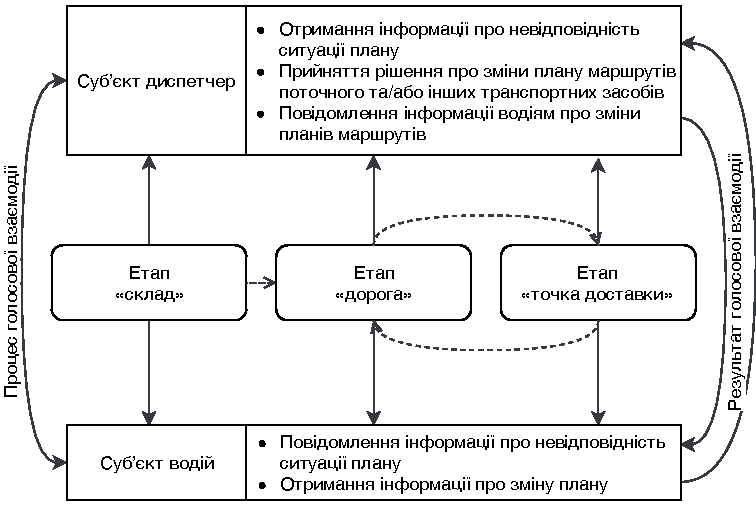
\includegraphics [width=.8\linewidth] {voice_interaction_schema}
  \caption{Модель голосової взаємодії суб’єктів дистрибуції}
  \label{img:voice_interaction_schema}  }
\end{figure}
\begin{multicols}{2}

Модель голосової взаємодії суб’єктів дистрибуції може бути зображена на схемі (рис. \ref{img:voice_interaction_schema}). Вона складається з трьох етапів, два останніх з яких, можуть циклічно повторюватися при наявності декількох точок доставки в маршруті. Стрілками позначено процеси голосової взаємодії, які можуть розгортатися на кожному з етапів при невідповідності плану та факту. У верхній та нижній частинах схеми показані принципові типи результатів голосової взаємодії для кожного з суб’єктів (диспетчера та водія). Ця логічна схема визначає принциповий алгоритм побудови дерева сценаріїв голосової взаємодії.

\section{Висновки}
Проведено аналіз вітчизняних та зарубіжних літературних джерел для пошуку шляхів використання можливостей голосового управління для оптимізації процесів дистрибуції по трьом напрямам: системи управління дистрибуцією, системи розпізнання голосу та системи голосової взаємодії.

Виявлено обмеження інструментів GPS контролю, які використовуються в системах управління дистрибуцією на етапі моніторингу доставки, але не відбивають причин відхилення реальної ситуації від запланованого маршруту. Саме на подолання цих обмежень має бути спрямована система голосової взаємодії в задачах управління дистрибуцією.

Наявні традиційні системи розпізнання голосу на основі нейронних мереж та прихованих Марківськіх моделей не забезпечують необхідний для задач дистрибуції рівень стійкості до шумів, багатодикторності та потребують потужного обладнання або стабільного доступу до інтернету.

Нові принципи розв’язання проблеми — перехід до іншої одиниці розпізнання мови (рефлексу або команди) та побудова дерева можливих сценаріїв взаємодії для зменшення кількості необхідних до розпізнання команд в залежності від контексту ситуації.

Таким чином, пропонується інтегративна рефлекторна модель голосової взаємодії в задачах управління дистрибуцією, в якій поєднується два сформульовані принципи: написання дерева можливих сценаріїв взаємодії та рефлекторна система голосового управління.

Перспективою подальшого дослідження є розробка програмного забезпечення, яке реалізуватиме запропоновану модель та інтегруватиметься з існуючою авторською системою автоматизації побудови маршрутів та управління дистрибуцією.
